%%%%%%%%%%		 If there is trouble with downloading packages used in this			%%%%%%%%%%
%%%%%%%%%%		 template, it is most likely because you have a relatively 			%%%%%%%%%%
%%%%%%%%%%		 old version of MikTex. The packages which might be troublesome 	%%%%%%%%%%
%%%%%%%%%%		 are \usepackage{textpos}, \usepackage{enumitem}, and posibly   	%%%%%%%%%%
%%%%%%%%%%		 \usepackage{enumitem}. If the problem occurs for you, I would		%%%%%%%%%%
%%%%%%%%%%		 suggest that you either reinstall MikTex or find your way			%%%%%%%%%%
%%%%%%%%%%		 working around this.												%%%%%%%%%%

\documentclass[20pt]{beamer}
\usepackage[orientation=portrait, size=a0, scale=2]{beamerposter}
\usepackage[utf8]{inputenc}
\usepackage{graphicx}
\usepackage{epsfig}
\usepackage[absolute,overlay]{textpos}
\usepackage[]{wrapfig}
\usepackage{color}
\usepackage{enumitem}
\usepackage[most]{tcolorbox}
\usepackage{tikz}
\usepackage[]{physics}

\usetikzlibrary{arrows.meta}
\usetikzlibrary{decorations.pathreplacing}
\usetikzlibrary{decorations.markings}
\usetikzlibrary{patterns}
\usetikzlibrary{3d}
\usetikzlibrary{math}
\usetikzlibrary{calc}

\definecolor{DarkBlue}{rgb}{0.1,0.1,0.5}
\definecolor{DarkYellow}{HTML}{FFCC00}
\definecolor{Red}{rgb}{0.9,0.0,0.1}
\setbeamercolor{wb}{fg=white,bg=DarkBlue}		% color of text + background in a beamercolorbox-box
\setbeamercolor{br}{fg=black,bg=Red}			% color of text + background in a beamercolorbox-box
\setbeamercolor{dd}{fg=DarkBlue,bg=DarkYellow}	% color of text + background in a beamercolorbox-box
\tcbset{on line,
        boxsep=4pt, left=0pt,right=0pt,top=0pt,bottom=0pt,
        colframe=white,colback=white,
        highlight math style={enhanced}
        }
\let\Textsize\normalsize
\def\Title#1#2{\center{\textcolor{black}{\scalebox{2.25}{\begin{tabular}{c@{}c@{}}
                \tcbox{#1}\\
                \tcbox{#2}
                \end{tabular}}}}}	%sets textcolor of main title
\def\Subtitle#1{\center{\textcolor{black}{\scalebox{1.5}{\colorbox{white}{#1}}}}}	% sets textcolor of main subtitle
\def\Head#1{\noindent{\Large\color{DarkBlue} #1}\bigskip\newline}
\def\Subhead#1{\noindent{\color{black} #1}}

\setbeamertemplate{navigation symbols}{}

\setbeamertemplate{background} 
{
        \begin{tikzpicture}
                \shade[top color=white, bottom color=blue, opacity=0.4] (0,0) rectangle(\paperwidth,
                \paperheight);
        \end{tikzpicture}
        \begin{tikzpicture}[xscale=12, yscale=4.5, overlay, xshift=-5.8cm, yshift=22.3cm]
            \tikzset{Ultra thick/.style={line width=5pt}}
            \draw[black, Ultra thick, opacity=0.6] node[anchor=north, xshift=4cm]{\Huge\(\ket{s, m_1}\)} (0,0) -- (4.9,3.4)
                    node[anchor=south, xshift=4cm]{\(\ket{s, m_2}\)};
            \draw[black, Ultra thick, opacity=0.6] (1, -0.3) -- (5,3.4);
            \draw[blue, Ultra thick, opacity=0.6, postaction=decorate, decoration={pre length = 1mm, post length = 1mm, markings, mark=
                        between positions 0.1 and 1 step
                        0.25 with {\pgftransformscale{2}\arrow{stealth}}}] plot [smooth, tension=1] coordinates {(-1,3.5) (1,1) (4,0)};
            \draw[blue, Ultra thick, opacity=0.6, postaction=decorate, decoration={pre length = 1mm, post length = 1mm, markings, mark=
                        between positions 0.1 and 1 step
                        0.4 with {\pgftransformscale{2}\arrow{stealth}}}] plot [smooth, tension=1] coordinates {(3,3.7) (3.5,2.5) (4.3,1.5)};
            \draw[blue, Ultra thick, opacity=0.6, postaction=decorate, decoration={pre length = 1mm, post length = 1mm, markings, mark=
                        between positions 0.1 and 1 step
                        0.28 with {\pgftransformscale{2}\arrow{stealth}}}] plot [smooth, tension=1] coordinates {(1,3.6) (2.5,1.5) (4.2,0.8)};
            \draw[blue, opacity=0.6] (4.2,0.8) node[anchor=west, xshift=2cm]{\Huge\(\va{B}\) };
        \end{tikzpicture}
}

\begin{document}
 \begin{frame}{}
%   document width from 0 to 16
%   usable width is between 0.5 and 15.5


  \begin{textblock}{2}(0.5,0.5) % {length of textblock}(x,y)
   
\epsfig{file=UU_logo, width=\textwidth} \\ [3mm]
  \end{textblock}

%  
%  
  \begin{textblock}{13}(2.5,0.5) 
   \Title{Simulating motion in synthetic magnetic}{monopole fields}
   \vspace{2.9cm}
   \Subtitle{}\\[8mm]
%  Chose one of the following two lines, comment out the other.
   %\Head{More stuff, for example your name}
   \Subhead{by Ola Carlsson, supervised by Erik Sjöqvist}
  \end{textblock}
%
%
  \begin{textblock}{15}(0.5,3.3)
   \begin{beamercolorbox}[wd=\textwidth, sep=8mm, left, rounded=true, shadow=true]{wb}
    Basic principle and premise
   \end{beamercolorbox}
   Magnetism always appears in dual form. Any size of ''magnet'' must have at least two poles, much like a common bar
   magnet has a north pole and a south pole. Imagine splitting such a bar magnet in twine, would two pieces of different
   magnetic ''charge'' be the result, one block of pure ''north'' and one of pure
   ''south''?    \begin{wrapfigure}{r}{0.4\textwidth}
           \centering
           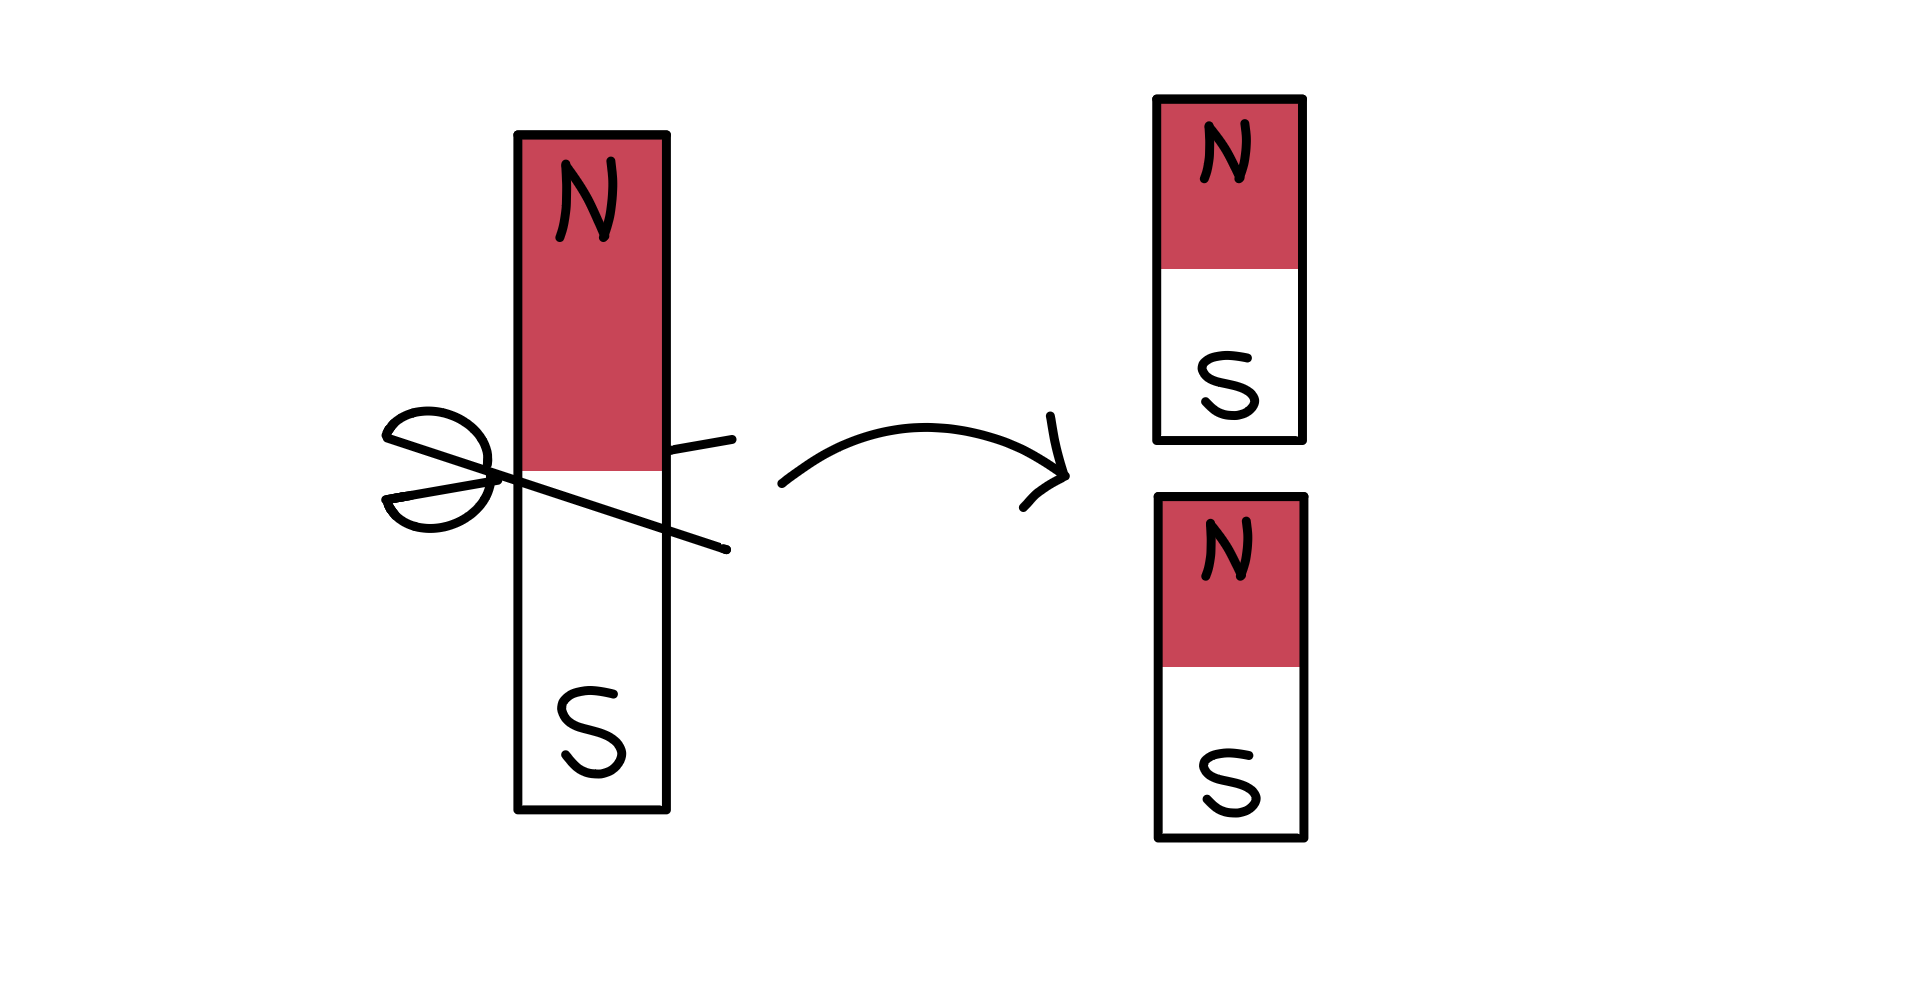
\includegraphics[width=0.37\textwidth]{magnetslice}
           \label{fig:magnets}
   \end{wrapfigure}
   That would be what is called magnetic monopoles, but such 
   things have yet never been observed, the bar magnet will split into two smaller bar
   magnets. 
   Other things in nature \textit{appear} to be monopoles even though they are not, and it
   is this kind of monopole which is studied here.
   This project concerns the modelling and simulation of a certain system with certain
   properties, such that its motion appears to be affected by a magnetic monopole.
  \end{textblock}
%
%
  \begin{textblock}{7.25}(0.5,7)
   \begin{beamercolorbox}[wd=\textwidth, sep=5mm, left, rounded=true, shadow=true]{br}
   The system and setup
   \end{beamercolorbox}
   \vspace{1cm}
    \begin{figure}[h]
        \centering
        \def\dgrid[####1](####2,####3)(####4)(####5)(####6){ %[draw options](corner)(distance in x)
        %(distance in y)(number of lines -1  per side)
        \foreach \x in {0,1,...,####6}{
                \pgfmathsetmacro\sx{\x*####4/####6}
                \draw[####1] (####2+\sx,####3) -- (####2+\sx,####3+####5);
                }
        \foreach \y in {0,1,...,####6}{
                \pgfmathsetmacro\sy{\y*####5/####6}
                \draw[####1] (####2,####3+\sy) -- (####2+####4, ####3+\sy);
                }
        }
        \begin{tikzpicture}[scale=3, decoration={markings, mark= between positions 0.1 and 1 step
                0.2 with {\arrow{stealth}}}, z={(90:10mm)},x={(-25:6mm)},y={(0:10mm)}]

            \tikzset{Ultra thick/.style={line width=7pt}}
            \begin{scope}[canvas is xy plane at z=0]
                \draw[black, Ultra thick, postaction={decorate}] (0,0) -- (6,0) -- (6,6) -- (0,6) -- cycle;
            \end{scope}
            \dgrid[red, dotted, very thick, canvas is xy plane at z=1](1,1)(4)(4)(8); %Draw the lab
            \dgrid[red, dotted, very thick, canvas is xy plane at z=5](1,1)(4)(4)(8);
            \dgrid[red, dotted, very thick, canvas is yz plane at x=1](1,1)(4)(4)(8);
            \draw[blue] (3,3,3) node[circle, fill, inner sep=6pt]{}; %Zerofield marker
            \dgrid[red, dotted, very thick, canvas is yz plane at x=5](1,1)(4)(4)(8);
            \dgrid[red, dotted, very thick, canvas is zx plane at y=1](1,1)(4)(4)(8);
            \dgrid[red, dotted, very thick, canvas is zx plane at y=5](1,1)(4)(4)(8);
            \begin{scope}[canvas is xy plane at z=6]
                \draw[black, Ultra thick, postaction={decorate}] (0,0) -- (0,6)
                        node[anchor=west, xshift=1cm, yshift=1cm, rotate=-25]{Current along arrows}
                        -- (6,6) -- (6,0) -- cycle;
            \end{scope}
            \draw[canvas is yz plane at x=6] (5,3) node{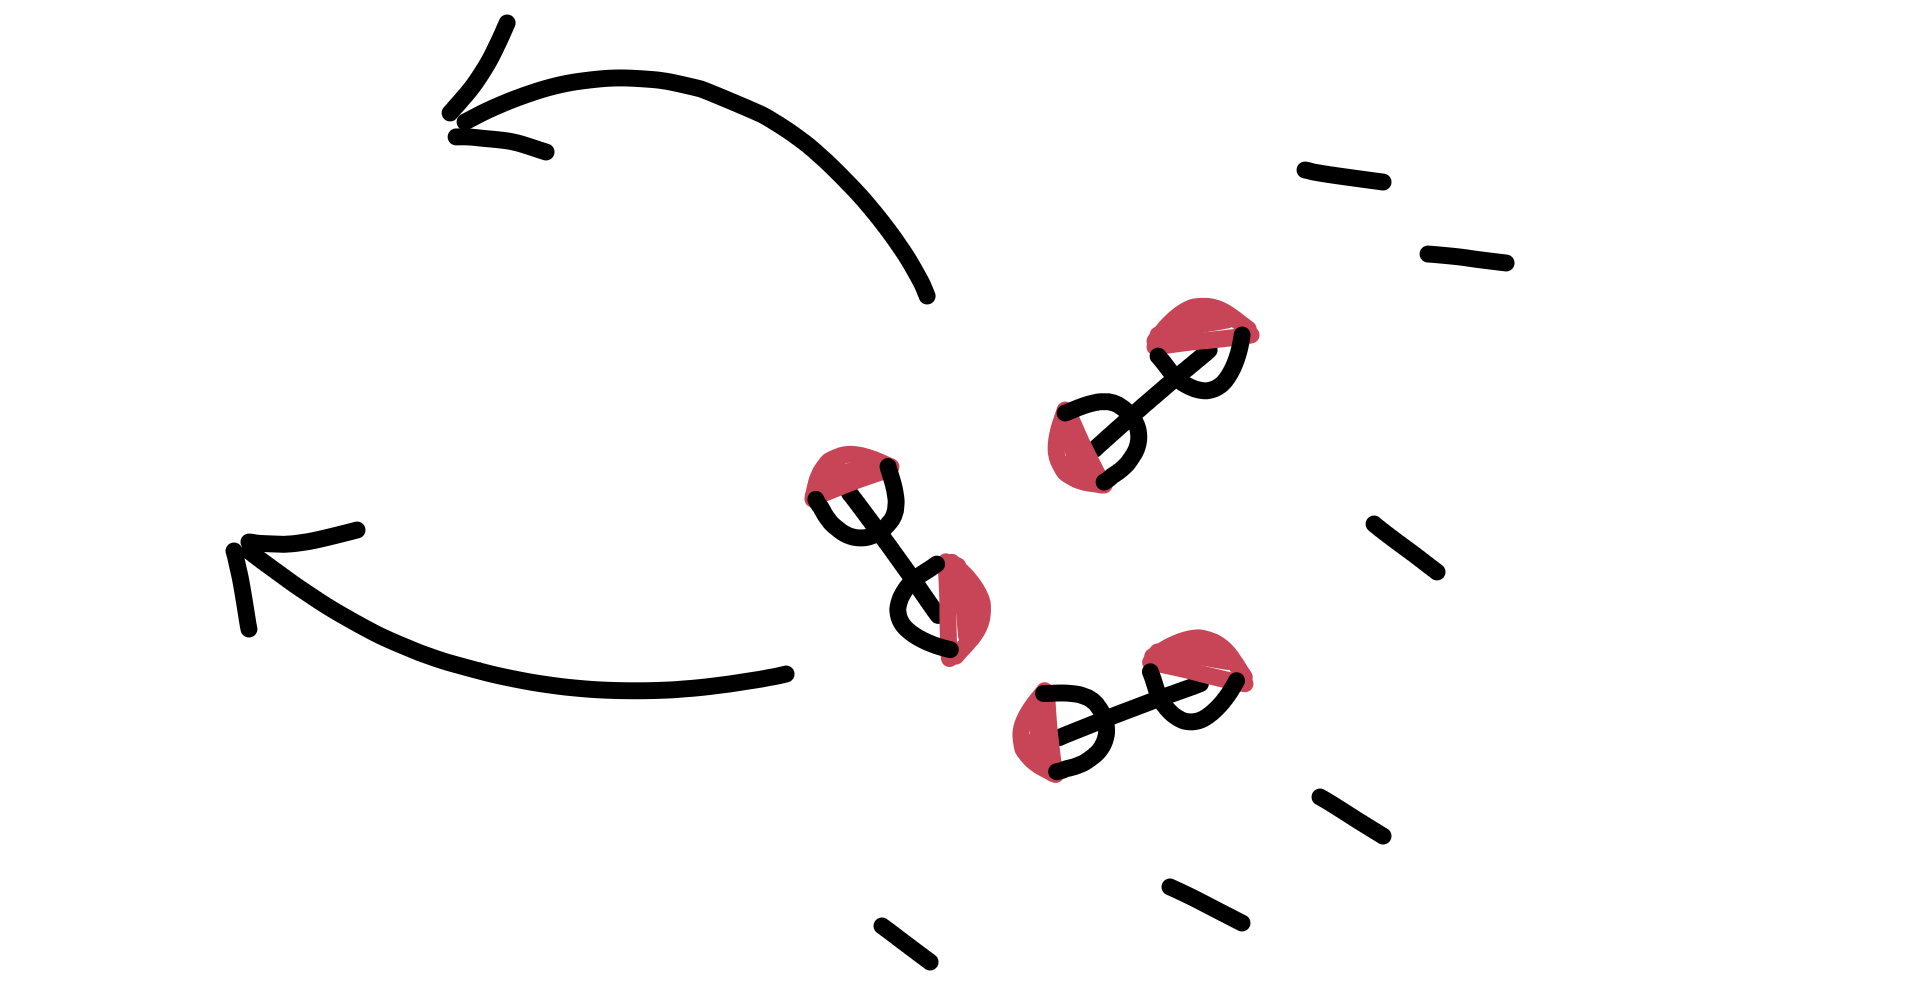
\includegraphics[scale=1.8]{dumbbellfly}};
        \end{tikzpicture}
        %\caption{\centering The currents generating the external magnetic field enclosing the
        %simulated ''lab'' region, shown in red. A blue dot marks the point of zero field
%strength at the centre.}
        \label{fig:extfield}
   \end{figure}
   \begin{itemize}[label=\textbullet, leftmargin=25mm]
           \item Consider two masses connected by a massless stick, like a 
                   dumbbell for weight lifting.
           \item Both masses have spin, a quantum bar magnet rotating about each end of
                   the dumbbell in a quirky ''quantum way''.
           \item The dumbbells are thrown into a magnetic field, how will they move and
                   rotate?
           \item Simulations were done for a magnetic field generated by two square coils,
                   as above.
           \item The red grid is the volume simulated.
           \item The blue dot marks a point of zero magnetic field, where a synthetic
                   monopole emits a synthetic magnetic
                   field.
           \item This synthetic field is \textbf{not} the ''regular'' field generated by
                   the coils.
           \item Both fields affect the dumbbell motion.
   \end{itemize}

  \end{textblock}
%
%
  \begin{textblock}{7.25}(8,7) 
   \begin{beamercolorbox}[wd=\textwidth, sep=5mm, left, rounded=true, shadow=true]{br}
   Results
   \end{beamercolorbox}
   \begin{itemize}[label=\textbullet, leftmargin=25mm]
           \item The effect of the monopole was shown for several sets of parameters. Blue
                   paths are without synthetic effects.
   \end{itemize}

   \begin{figure}[h]
           \centering
           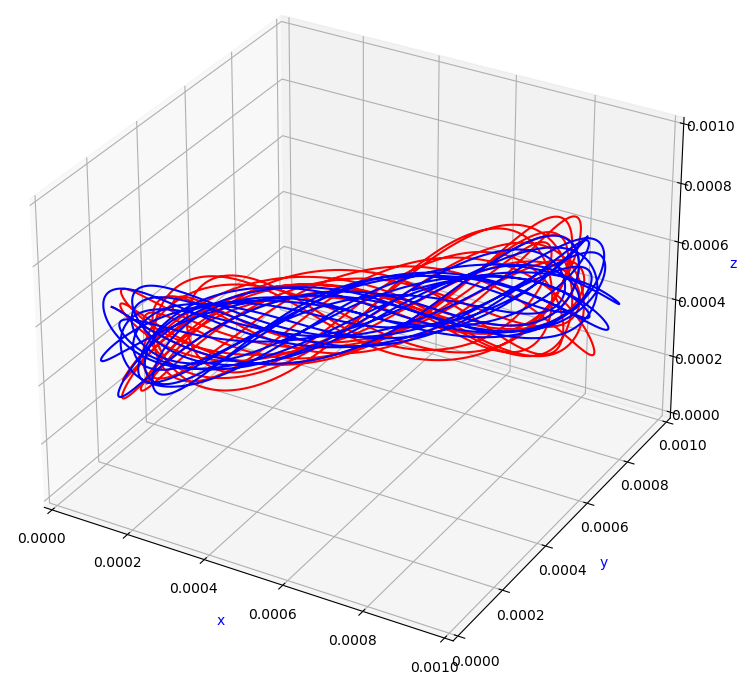
\includegraphics[width=0.6\textwidth]{(0,2)-comp1}
           \label{fig:comp2}
   \end{figure}
   \begin{itemize}[label=\textbullet, leftmargin=25mm]
           \item Placing the dumbbell in a high energy state traps it between the coils, as
               shown here.
   \end{itemize}
   \begin{figure}[h]
           \centering
           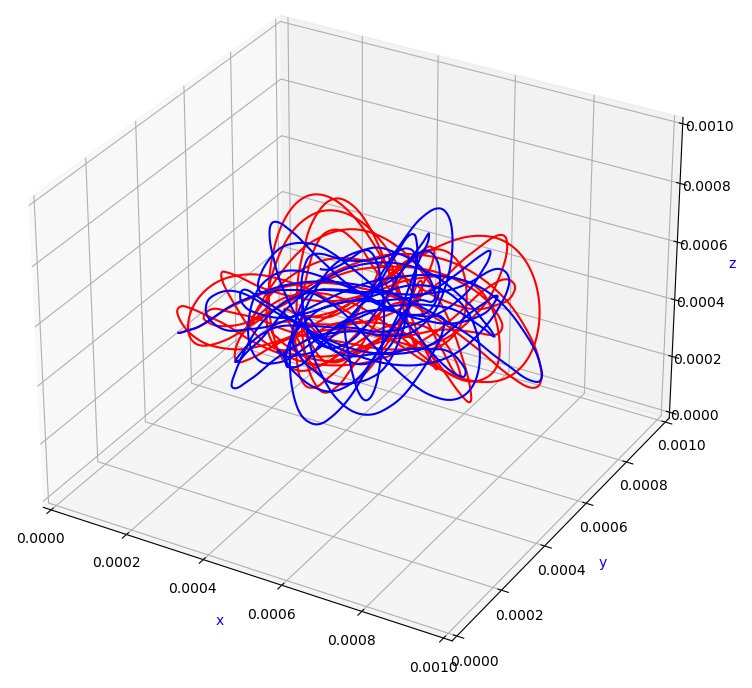
\includegraphics[width=0.6\textwidth]{(1,1)-comp1}
           \label{fig:comp1}
   \end{figure}
   \begin{itemize}[label=\textbullet, leftmargin=25mm]
           \item Lower mass means more synthetic effects, as in the lower plot.
   \end{itemize}

  \end{textblock}



 \end{frame} 
\end{document}
